\documentclass{article}
\usepackage[utf8]{inputenc}

%\usepackage{sectsty}
\usepackage{fancyhdr}
\usepackage[top=1.25cm, bottom=2cm, left=2cm, right=2cm]{geometry}
%\usepackage{tabularx,tabulary}
\usepackage{graphicx}
\date{3 Avril 2019}
\author{FRANCESCHETTI Maël\\KADOCH Daoud\\MANSON Fabien\\CASTANET Nicolas}
\title{\LARGE{Projet 3i013\\}Rapport de Projet}

\usepackage[french]{babel}
%\usepackage[utf8x]{inputenc}
%\usepackage{amsmath}
%\usepackage[colorinlistoftodos]{todonotes}
\begin{document}

\begin{titlepage}

\newcommand{\HRule}{\rule{\linewidth}{0.5mm}} % Defines a new command for the horizontal lines, change thickness here

\center % Center everything on the page
 
%----------------------------------------------------------------------------------------
%	HEADING SECTIONS
%----------------------------------------------------------------------------------------

\textsc{\LARGE Université Pierre-et-Marie-Curie}\\[3cm] % Name of your university/college
\textsc{\Large Licence Informatique 3\up{ème} Année}\\[0.5cm] % Major heading such as course name
\textsc{\large Projet 3i013}\\[2cm] % Minor heading such as course title

%----------------------------------------------------------------------------------------
%	TITLE SECTION
%----------------------------------------------------------------------------------------

\HRule \\[0.4cm]
{ \huge \bfseries Rapport de Projet}\\[0.4cm] % Title of your document
\HRule \\[2cm]
 
%----------------------------------------------------------------------------------------
%	AUTHOR SECTION
%----------------------------------------------------------------------------------------

\begin{minipage}{0.4\textwidth}
	\begin{flushleft} \large
	\emph{Auteurs:}\\[0.2cm]
	Nicolas \textsc{CASTANET}\\ % Your name
	Maël \textsc{FRANCESCHETTI}\\ % Your name
	Daoud \textsc{KADOCH}\\ % Your name
	Fabien \textsc{MANSON} % Your name
	\end{flushleft}
\end{minipage}
~
\begin{minipage}{0.4\textwidth}
	\begin{flushright} \large
	\emph{Enseignant:} \\[0.2cm]
	Fabrice \textsc{KORDON}
	\end{flushright}
\end{minipage}\\[4cm]

%----------------------------------------------------------------------------------------
%	DATE SECTION
%----------------------------------------------------------------------------------------

{\large 3 Avril 2019}\\[3cm] % Date, change the \today to a set date if you want to be precise

%----------------------------------------------------------------------------------------
%	LOGO SECTION
%----------------------------------------------------------------------------------------


\includegraphics[scale=0.15]{logo_sorbonne.png} % Include a department/university logo - this will require the graphicx package
 
%----------------------------------------------------------------------------------------

\vfill % Fill the rest of the page with whitespace

\end{titlepage}

% -----------------------------------------------------
\newpage
\renewcommand{\contentsname}{\center{Table des Matières}\vspace*{5cm}}

\tableofcontents



\newpage
\section{Présentation du Projet}
	\subsection{Contexte}
		Un client souhaite effectuer un vol autonome avec un drone Bebop 2 tout en visualisant sur un iPod Touch le retour vidéo de la caméra embarquée sur le drone. L'iPod sera placé dans un masque de vue à la première personne. \\	
		%Le client souhaite faire effectuer des vols autonomes à un drone Bebop 2, avec un retour vidéo en temps réel sur un iPod Touch. Ce dernier pourra être placé dans un masque de vue à la première personne.\\
		La solution devra permettre à l'utilisateur de saisir un plan de vol sur une carte interactive et de le faire exécuter par le drone tout en ayant un retour vidéo sur l'iPod.\\
		
        

	\subsection{Solutions étudiées}
		%\vspace*{0.3cm}
		\begin{enumerate}
        	\item 
        	\item 
		\end{enumerate}
		
	\newpage
	\subsection{Use Case}	
	    \subsubsection{Création d'un plan de vol}
	    Dans le premier cas d'utilisation, l'utilisateur souhaite créer un nouveau plan de vol afin de le faire suivre à son drone dans le futur, voici les étapes qu'il va suivre:
	    
	    \vspace{0.7cm}	     
	    \begin{center}
	    \renewcommand{\arraystretch}{2}
        \begin{tabularx}{15cm}{|c|X|}
            \hline
            1 & L'utilisateur lance l'application et arrive sur la page d'accueil.\\
            \hline
            2 & L'utilisateur lance la fonctionnalité de saisie du plan de vol sur une machine connectée au réseau local.\\
            \hline
            3 & L'utilisateur saisit le plan de vol sur la carte en spécifiant les points de passage du drone ainsi que les altitudes que le drone doit adopter au cours du vol. \\
            \hline
            4 & L'utilisateur valide la saisie de son plan de vol, ce dernier est enregistré. \\
            \hline
        \end{tabularx}
        \end{center}
        
	    \vspace{0.8cm}
	    
	    \subsubsection{Exécution d'un plan de vol}
	    Dans le deuxième cas d’utilisation, l'utilisateur possède déjà un ou plusieurs plan de vol enregistrés sur sa machine, par exemple le tour de son énorme jardin qu'il souhaite surveiller sans avoir à ce déplacer. Il fais désormais exécuter au drone l'un de ces plan de vol et observe le retour vidéo sur son Ipod.
	    Voici les étapes suivient :
	    
	    \vspace{0.7cm}	     
	    \begin{center}
	    \renewcommand{\arraystretch}{2}
        \begin{tabularx}{15cm}{|c|X|}
            \hline
            1 & L'utilisateur lance l'application et arrive sur la page d'accueil.\\
            \hline
            5 & L'utilisateur allume le drone et y connecte sa machine en wifi. \\
            \hline
            6 & L'utilisateur lance la fonctionnalité d'exécution du plan de vol. \\
            \hline
            7 &  L'utilisateur démarre l'iPod touch, le connecte au réseau local et lance l'application de réception vidéo. La réception vidéo en temps réel sur l'iPod commence.\\
            \hline
            8 & L'utilisateur sélectionne parmi les plans de vols présents sur le drone celui qu'il souhaite réaliser. \\
            \hline
            9 & L'utilisateur place l'iPod dans le masque FPV, le met sur sa tête, puis lance l'exécution du plan de vol. Le drone décolle. \\
            \hline
            10 & Le drone effectue le plan de vol choisi, l'utilisateur voit en temps réel ce que le drone filme et peut constater l'état d'enneigement de son jardin. \\
            \hline
            11 & L'utilisateur attend la fin de l'exécution du plan de vol pour retirer le masque et aller récupérer le drone une fois qu'il aura atterri à son point de départ, comme prévu.\\
            \hline 
\end{tabularx}
        \end{center}
	    
	    
	\newpage
	\subsection{Rappel du cahier des charges}
    Nous rappelons ici les princpaux points du cahier des charges dans cette section.
    Les besoins fonctionnels et le diagramme des fonctionnalités se trouvent dans le cahier des charges.
    
    \subsubsection{Périmètre}
    \textbf{À qui s'adresse le produit ?}
    \newline
	Ce projet est destiné à un public désirant effectuer une ronde d'une durée de 20 à 25 minutes maximum avec son drone.\\
		La portée maximale du drone est de 200 mètres pour une altitude de 100 mètres tout au plus.\\
	\newline
	\textbf{Les Limites}
	\newline
		Le drone ne sera pas capable d'éviter les obstacles durant sa ronde, c'est à l'utilisateur d'établir un trajet cohérent avec son environnement.\\
		De plus, dans le cas où le trajet proposé est trop long par rapport à l'autonomie du drone, un simple message d'avertissement sera affiché pour prévenir l'utilisateur, l'application ne sera pas en mesure d'empêcher cette ronde.
	

    
    \subsubsection{Ressources}
    \textbf{Nous rappelons ici le matériel à notre disposition pour la réalisation du projet :}

	\begin{enumerate}
        \item Un drone Bebop 2.
        \item Un iPod Touch de 6ème génération sous iOS 12.
        \item Un accès aux salles machines SAR équipées de machines sous OSX.
        \item Un accès aux salles informatiques équipées de machines sous Linux.
    \end{enumerate}
    \vspace{0.1cm}
        L'équipe est composée de quatre étudiants en troisième année de licence d'informatique.\\
        Nos connaissances en programmation sous Linux sont bonnes mais le langage Objective-C et l'univers iOS nous sont pour le moment encore inconnus.
        
    \subsubsection{Objectifs négociés}
    Après avoir éxaminé la demande du client et retenue une solution matérielle, les objectifs suivants ont été formulés dans le cahier des charges :
		\vspace{0.1cm}
	\begin{enumerate}
        	\item Permettre à l'utilisateur de saisir un plan de vol étape par étape sur une carte interactive et de spécifier les altitudes du drone à chaque point de passage.
        	\item Permettre à l'utilisateur de sauvegarder son plan de vol pour le réutiliser plus tard.
			\item Permettre à l'utilisateur de lancer l'exécution du plan de vol réalisé au préalable.
		 	\item Rediriger le flux vidéo du drone vers l'iPod Touch. 
		 	\item Minimiser les latences vidéo (de l'ordre de la seconde).
		 	\item Permettre d'arrêter le vol en cours en cas d'urgence.
    \end{enumerate}
        
    
        
	

		
	\newpage
\section{Architecture Logicielle}
    \subsection{Interface utilisateur}
    L'interface utilisateur est une interface GTK permettant d'intéragir avec le SDK Parrot afin d'enregistrer des trajets sur le drone et de les exécuter.
    \newline
    Elle permet également d'intéragir avec le Serveur local afin de saisir intéractivement le plan de vol à l'aide de l'application javascript et de créer les fichiers Mavlink.
    \vspace{0.2cm}
    \newline
    Voici l'architecture d'intéraction de l'interface utilisateur:
        \vspace*{0.5cm}
        \begin{center}
		\begin{figure}[!h]
		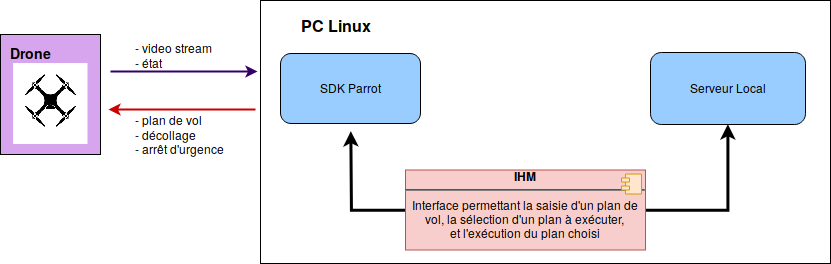
\includegraphics[scale=0.5]{Rapport/new_HIM.png}\\
		 \vspace*{0.3cm}
		\caption{Interface utilisateur}
		\end{figure}
        \end{center}

\newpage
        
	 \subsection{Controle du drone}
	 Le controle du drone est axé autour de la génération du fichiers mavlink à l'aide de l'application JS sur le serveur local et du SDK Parrot qui permet d'envoyer des commandes au drone et de connaitre son état.
	 \newline
	 Apres voir saisie intéractivement un trajet à l'aide de l'application javascript, le fichier Mavlink généré et envoyé au SDK Parrot. 
	 \vspace{0.1cm}
	 \newline
	 
	 Le SDK permet ensuite le controle du drone à savoir:
	 \begin{enumerate}
        	\item Connexion au drone.
        	\item Exécution d'un plan de vol.
			\item Arrêt d'urgence.
    \end{enumerate}
    Le décolage et l'arrêt d'urgence du drone sont des commandes envoyés directement par le serveurs, ses commandes seront envoyés au serveur par l'IPod afin de permettre un décolage et un arrêt ergonomique.
    \vspace{0.2cm}
    \newline
    Il permet égaement la réception de l'état du drone et du flux vidéo qui sera par la suite traité avec FFMPEG et envoyé en RTP à l'Ipod.
    
	    \vspace*{0.3cm}
	    \begin{center}
		\begin{figure}[!h]
		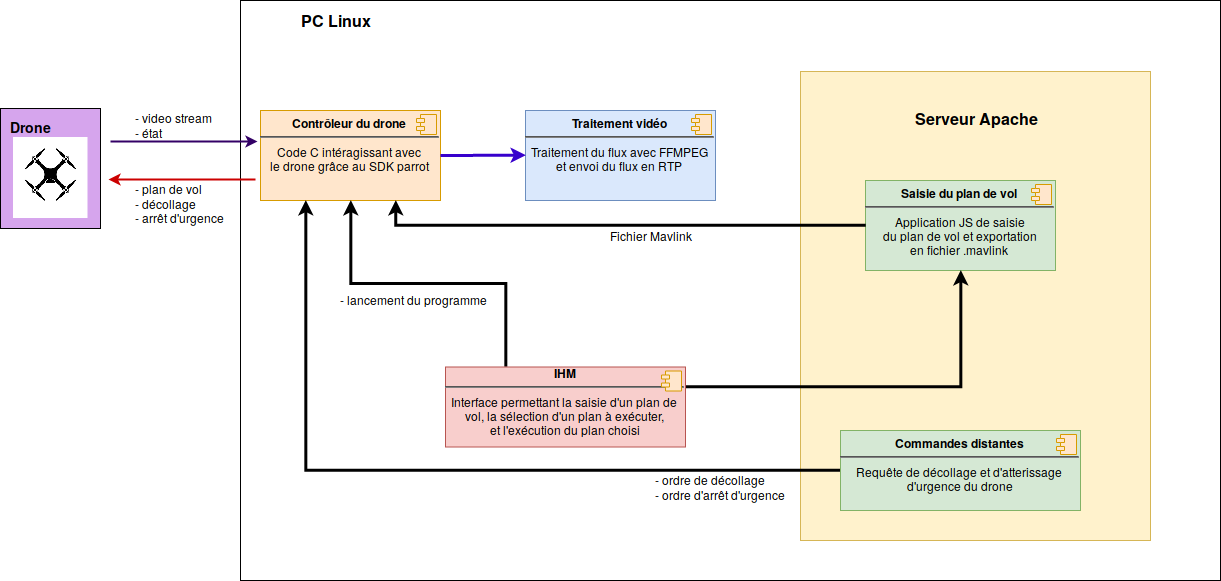
\includegraphics[scale=0.4]{Rapport/new_controle_drone.png}\\
		\caption{Controle du drone}
		\end{figure}
        \end{center}
		
     \newpage
     \subsection{Application IOS}
     L'application IOS permet d'afficher le flux vidéo du drone et d'envoyés des requetes au serveur en effectuant des gestes simples avec l'Ipod afin de démarrage du drone et d'effectuer l'arrêt d'urgence.
     \vspace{0.2cm}
     \newline
     Dans un premier temps, l'application scanne le réseau afin de se connecter au serveur local.
     Apres la connection une requete de demande de description du flux vidéo au format SDP est automatiquement envoyé au serveur.
     \vspace{0.2cm}
     \newline
     Le descripteur de flux est alors retourné par le serveur à l'application IOS, en parrallèle, elle reçoit également le flux video grâce au protocol RTP, le SDK VLC permet ensuite l'affichage vidéo.
        \vspace*{0.3cm}
	    \begin{center}
		\begin{figure}[!h]
		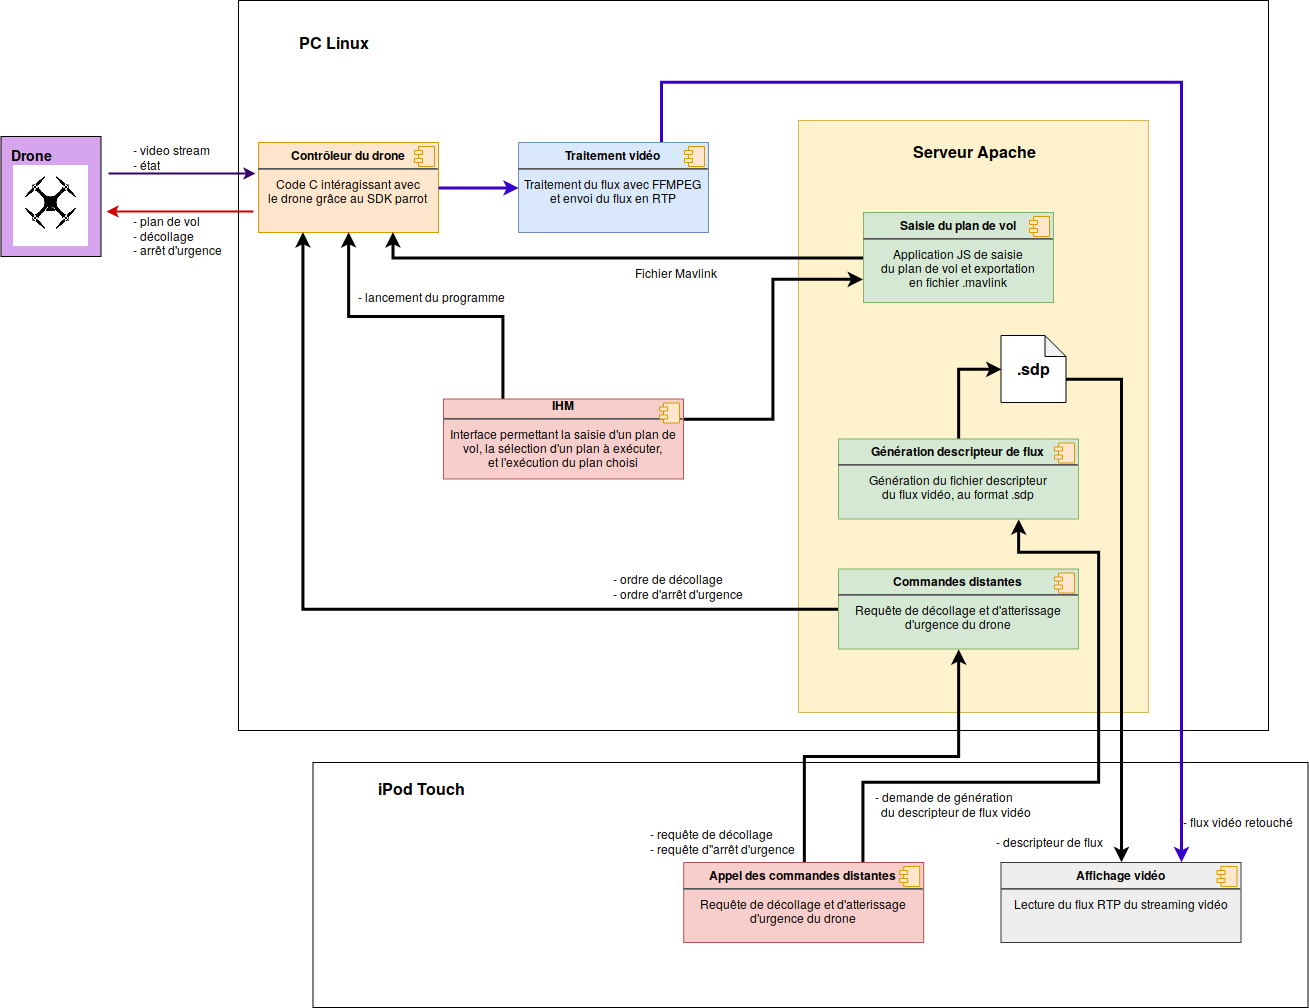
\includegraphics[scale=0.4]{Rapport/new_archi_logicielle.png}\\
		\caption{Application IOS}
		\end{figure}
        \end{center}
        
    \newpage
	
	\subsection{Architecture logicielle globale}
	    \vspace*{0.3cm}
	    \begin{center}
		\begin{figure}[!h]
		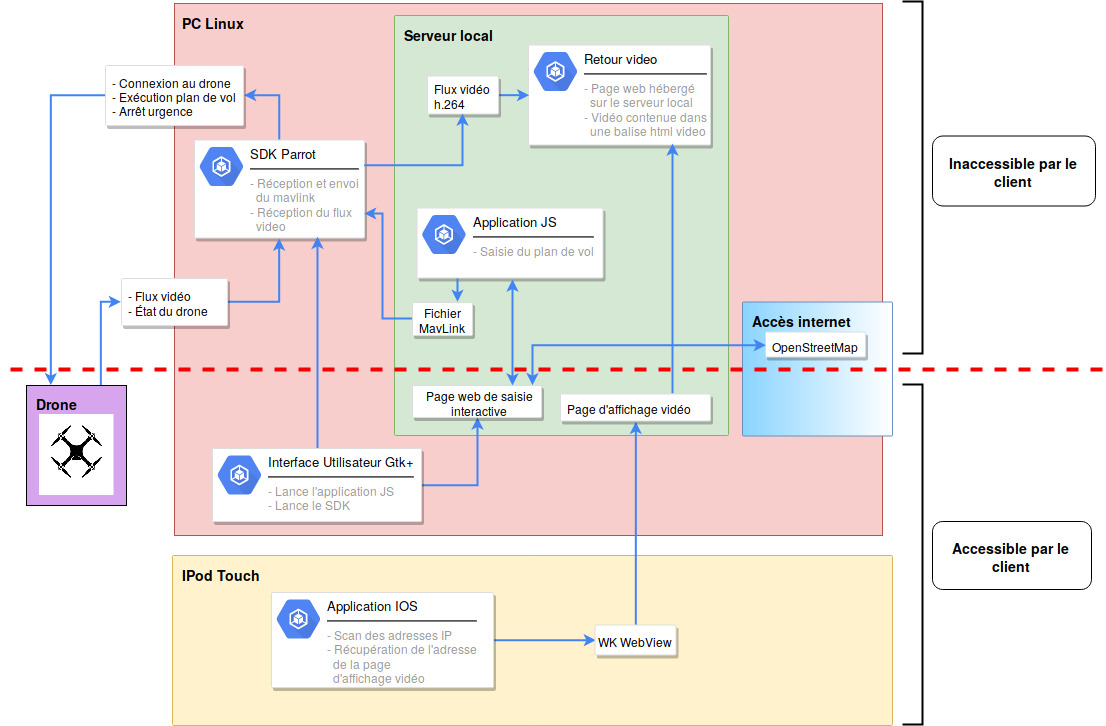
\includegraphics[scale=0.47]{Rapport/Architecture_logicielle_v2.jpg}\\
		\caption{Architecture logicielle}
		\end{figure}
        \end{center}
		
\newpage
\section{Problèmes rencontrés}
	\subsection{Problèmes matériels}
		
	
	\subsection{Solutions}
	
	

\newpage
\section{Organisation du travail}
	\subsection{Diagramme de Gantt}
        
	\subsection{Répartition des taches}
	
\section{Déploiement}


\newpage
\section{Comparatif aux objectifs fixés}
	
\newpage
\section{Améliorations possibles}


\newpage
\section{Conclusion}
	
 
\end{document}